\documentclass{article}
\usepackage[utf8]{inputenc}
\usepackage[T1]{fontenc}
\usepackage{textcomp}
\usepackage{amsmath,amssymb}
\usepackage{lmodern}
\usepackage[a4paper]{geometry}
\usepackage{graphicx}
\usepackage{xcolor}
\usepackage{microtype}
\usepackage{hyperref}
\usepackage{diagbox}
\usepackage{booktabs}
\usepackage{listings}
\usepackage[francais]{babel}
\definecolor{darkWhite}{rgb}{0.94,0.94,0.94}
\lstset{
  aboveskip=3mm,
  belowskip=-2mm,
  backgroundcolor=\color{darkWhite},
  basicstyle=\footnotesize,
  breakatwhitespace=false,
  breaklines=true,
  captionpos=b,
  commentstyle=\color{red},
  deletekeywords={...},
  escapeinside={\%*}{*)},
  extendedchars=true,
  framexleftmargin=16pt,
  framextopmargin=3pt,
  framexbottommargin=6pt,
  frame=tb,
  keepspaces=true,
  keywordstyle=\color{blue},
  language=C, JavaScript
  literate=
  {²}{{\textsuperscript{2}}}1
  {⁴}{{\textsuperscript{4}}}1
  {⁶}{{\textsuperscript{6}}}1
  {⁸}{{\textsuperscript{8}}}1
  {€}{{\euro{}}}1
  {é}{{\'e}}1
  {è}{{\`{e}}}1
  {ê}{{\^{e}}}1
  {ë}{{\¨{e}}}1
  {É}{{\'{E}}}1
  {Ê}{{\^{E}}}1
  {û}{{\^{u}}}1
  {ù}{{\`{u}}}1
  {â}{{\^{a}}}1
  {à}{{\`{a}}}1
  {á}{{\'{a}}}1
  {ã}{{\~{a}}}1
  {Á}{{\'{A}}}1
  {Â}{{\^{A}}}1
  {Ã}{{\~{A}}}1
  {ç}{{\c{c}}}1
  {Ç}{{\c{C}}}1
  {õ}{{\~{o}}}1
  {ó}{{\'{o}}}1
  {ô}{{\^{o}}}1
  {Õ}{{\~{O}}}1
  {Ó}{{\'{O}}}1
  {Ô}{{\^{O}}}1
  {î}{{\^{i}}}1
  {Î}{{\^{I}}}1
  {í}{{\'{i}}}1
  {Í}{{\~{Í}}}1,
  morekeywords={*,...},
  numbers=left,
  numbersep=10pt,
  numberstyle=\tiny\color{black},
  rulecolor=\color{black},Usine logicielle javascript
  showspaces=false,
  showstringspaces=false,
  showtabs=false,
  stepnumber=1,
  stringstyle=\color{gray},
  tabsize=4,
  title=\lstname,
}
\hypersetup{pdfstartview=XYZ}
\title{Réseaux}
\author{}
\date{}
\begin{document}
\maketitle{}
\tableofcontents
\newpage
\section*{{\underline{Modalité d'examen}}}
L'UE de réseaux est à 3 ECTS (Système européen de transfert et d'accumulation de crédits). \\
L'évaluation se fera en contrôle continue. \\
Ecrit(Après les vacances de Toussaint) -> 50\% \\
TP noté -> 25\% \\
Projet (TP) -> 25\% \\

 

\section{\underline{Introduction}}
Lorsqu’on souhaite communiquer avec plusieurs machines par intermédiaire d’un ou plusieurs réseaux, on soit pouvoir disposer d’un ensemble de fonctionnalités qui permettent les échanges. \\
Elle est rendue obligatoire par la nature diverse des réseaux qui sont utilisés. \\ 
- Téléphonie cuivre (ADSL) \\
- Téléphonie Mobile (3g/4g/5g) \\
- Wifi \\
- Fibre \\
On a besoin d’une approche unifiée. \\

\newpage 
\section{\underline{Modèle en couche OSI}}
\subsection{Le modèle}
Le modèle OSI (pen System Interconnection) est théorique. il a été introduit par l’ISO (International Standard Organisation) et définit les fonctionnalités nécessaire pour interconnexion. \\ 
Le modèle dispose de 7 couches : \\
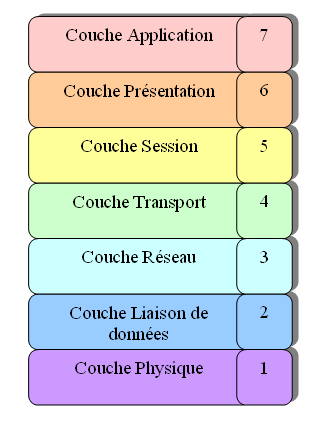
\includegraphics{image/modeleOSI.PNG} \\
\url{https://sites.google.com/site/6hyperyon9/reseau/modele-osi}
\\
\\
\subsubsection*{1- La couche physique}
Concerne les médias de communication. \\ 
- Cable Ethernet \\
- Signal Radio Wifi \\
- Signaux lumineux sur la fibre \\
\subsubsection*{2- La couche liaison de données}
Adressage physique \\
Taille des messages qui transitent sur les réseaux physique \\
\newpage 
\subsubsection*{3- La couche réseau}
Gère la communication de proche en proche \\ 
- Permet un adressage logique \\
- Décorrélé de la couche liaison (IP/ICMP) \\
\subsubsection*{4- La couche transport}
Gère la communication de bout en bout. \\
- TCP/UDP \\
- Notion de port \\
\subsubsection*{5- La couche session}
Notion d’identification (RCP/PPTP/…)
\subsubsection*{6- La couche présentation}
S’occupe du codage des données \\
- Données crypter (SSL/TLS/…) [Si site sécurisé) \\
\subsubsection*{7- La couche application}
Ce qu’on programme \\
-HTP \\
-DNS \\

\newpage
\subsection{Principe de fonctionnement}
Une machine A veut envoyer un message à une machine B. \\
Le messages est en-capsulé dans la couche 6. \\
Le message descend et est en-capsulé dans le niveau en dessous jusqu’à atteindre le niveau 1. \\
Où le message est envoyé et transite par le réseaux. Quand il arrive sur B le message décapsulé jusqu’à atteindre le niveau 7. \\  
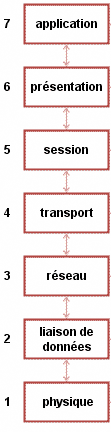
\includegraphics{image/modele_OSI.png} \\ 
\url{https://openclassrooms.com/fr/courses/857447-apprenez-le-fonctionnement-des-reseaux-tcp-ip/854659-le-routage}
\\
Remarque : Dans le modèle OSI, les couches sont indépendantes les unes des autres.
\subsection{Avantage et inconvénients}
\subsubsection*{Avantages}
Les couches ont des champs d’actions bien délimiter donc on peut facilement changer le protocole utilisé à l’intérieur d’une couche. \\
Ça va limiter l’impact des modification qu’on veut faire quand on change de protocole. \\
Permet une plus grande modularité \\
\subsubsection*{Inconvénients}
Par le phénomène d’encapsulation, la taille des données peut rapidement devenir assez grandes. \\
Difficile de configurer les niveaux les plus bas. \\

\section{\underline{Protocole IP}}
Le protocole IP se situe au niveau 3 du modèle OSI et son but est de permettre l’interconnexion de plusieurs réseaux de nature différentes . \\
Il permet un détachement du réseau physique. \\
Le protocole IP comprend 3 fonctionnalités : \\
- Adressage logique \\
- Une façon de router les paquets \\
- Une remise émission des paquets \\
\\
Il existe deux versions du protocole en usage IPv4 et IPv6.
\\
\subsection{Adressage IP}
Chaque hôte relié au réseau dispose d’une adresse IP unique. \\
Une IP peut être donnée de manière permanente ou de manière dynamique. \\ 
\\
Sur IPv4 les adresses sont codées sur 32 bits – 4 octets. \\
Sur IPv6 les adresses sont codées sur 128 bits. \\
\\
Pour l'IPv4, il y a une façon de représenter les adresses en notations pointées (a.b.c.d avec a,b,c,d compris entre 0 et 255). \\
\\
\newpage
Exemple : \\
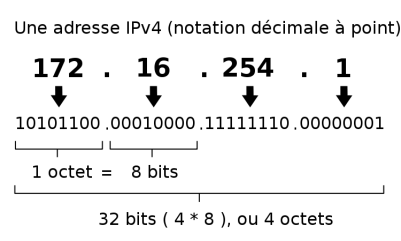
\includegraphics{image/IPv4.png} \\
\\
\url{http://math.univ-lyon1.fr/irem/Formation_ISN/formation_reseau/couche_reseau/adressage_ip.html}
\\
\newpage
L’adresse IP est constituée de deux partie : \\
- Adresse réseau \\
- Adresse machine \\
\\
\subsection{Les classes d'adresses}
Il y a 5 classes d’adresses : \\
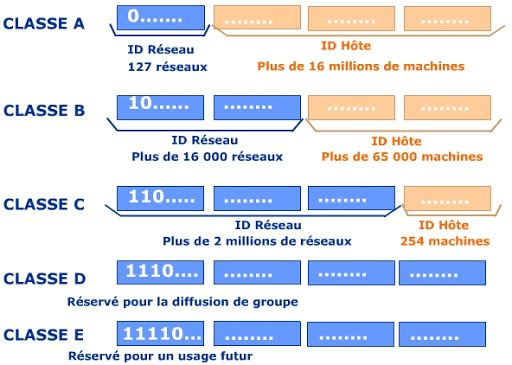
\includegraphics{image/classesIP.jpg} \\
\url{http://wapiti.enic.fr/commun/ens/peda/options/ST/RIO/pub/exposes/exposesrio2002/andre-pelloux/penurieadresses.htm} \\
\\
Remarque : Pour déterminer la classe regarder les premiers bits suffit. \\
A 1.0.0.0 → 126.0.0.0 \\
B 128.1.0.0 → 191.255.0.0 \\
C 192.0.1 → 233 255 0 \\
D 224.0.0.0 → 235 255 255 255 \\

\newpage
\subsection{Les adresses spéciales}
\subsubsection{Adresse locale}
127.0.0.1 → Boucle locale qui correspond à l’adresses de la machine locale(Même si connecté à aucun réseau) | Programmation native (exemple : Adresse de BDDs) permet d’avoir le même programme qu’on soit connecté ou pas.
\subsubsection{Adresse de broadcast}
\subsubsection*{Si adresse = 0}
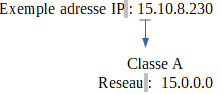
\includegraphics{image/B1.png}
\subsubsection*{Si l'adresse est composé seulement de 1 bit}
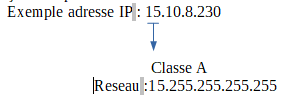
\includegraphics{image/B2.png}\\
Le message est adressé à toutes les machines connectées au réseau concerné.
\subsubsection*{Broadcast universel}
255.255.255.255
ça concerne tous les ordinateurs connectés au réseau sur lequel on est même si on ne connaît pas notre adresse réseau.
\subsubsection*{Si Adresse réseau est = 0}
Correspond au réseau sur lequel je suis connecté.

\subsubsection{Les adresse privées}
Ce sont des adresses qui son non routables. \\
Elle est utilisable seulement sur un réseau local (domestique, entreprise, …). \\
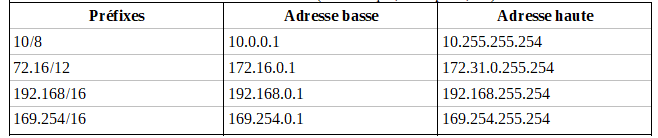
\includegraphics{image/adresse_pv.png}

\subsection{Structure des paquets IP}
L’unité de base qui va être envoyée sur le réseau un paquet IP (ou datagramme) prend la forme d’une donnée qui est très structurée. \\

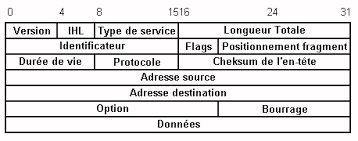
\includegraphics{image/data_ip.png} \\
\\
\url{http://home.scarlet.be/vinderick.pascal/reseaux_wan/protocoles/tcp_ip/datagramme%20ip.htm} \\
\\ 
Le plus petit datagramme fait 20 octets. \\

\subsubsection*{1- Version du protocole IPv4 ou IPv6}
Détermine comment le reste de la donnée doit être traité. \\

\subsubsection*{2- IHL ou La longueur d’en tête}
Exprimée en mots de 32 bits

\subsubsection*{3- Type de service}
Indique comment le datagramme doit être gérée pour le/les routeur(s). \\
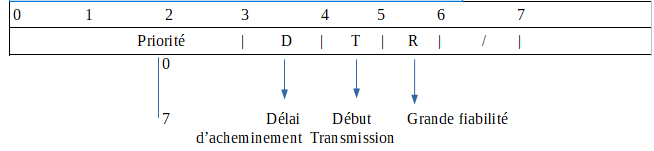
\includegraphics{image/Type.PNG}

\subsubsection*{4- Longueur totale}
Exprimée en octets (max $2^{16}$ )

\newpage
\subsubsection*{5- Flags}
Autorisation de fragmentation (Exemple : DNF)

\subsubsection*{6- Durée de vie TTL (Time to live)}
A chaque fois que l’on passe sur un routeur le TTL décrémente d’une unité. \\
Si le TTL atteint la valeur 0, le routeur qui constate cette valeur le supprime et envois un message d’erreur ICMP à l’expéditeur. \\
\textit{(Commande pour le TP1 : "ping" permet de savoir si un ordinateur est atteignable)}

\subsubsection*{7- Protocole}
Protocole du message (TCP, UDP/ICMP)

\subsection{Fragmentation}
Conceptuellement un datagramme IP est un morceau de message qui va de l’expéditeur jusqu’au destinataire. \\
Le datagramme est amené à traverser des réseaux physique avec des capacité de « trames » varaibes et différentes d’un réseau à l’autre. \\
MTU : Maximum transfert unit. \\  
Si le MTU du réseau est plus petit que la taille du datagramme à envoyer, on doit réduire la taille. C’est le phénomène de fragmentation. \\
La taille maximum d’un datagramme IP est 65536. Le MTU peut être beaucoup plus faible sur le réseau physique. \\
\subsubsection*{Exemple} \\
\emph{Photo à insérer} \\ 
\\
On fait l'hypothèse raisonnable que l'en-tête occupe 20 octets. \\ 
\\
Comment réunir les fragments issus d'un même datagramme ? \\
\\
Pour faire l’identification des datagramme, la machine A affecte un identifiant unique à chaque datagramme. 
Les nouveaux fragments  qu’on crée vont avoir ce même identifiants. \\
\\
Flags : Message à suivre ? 1 ou 0 \\
\\
\newpage
L'identifiant va permettre de remettre les morceaux ensembles. \\
\\ 
- champ décalge (offset) qui correspond déplacement au décalage en nombre d'octets dans le message initial.\\►

\begin{tabular}{|c|c|} 
\hline 
20 & 1600 \\ 
\hline 
\end{tabular}
\\ Il est nécessaire de fragmenter \\
Les en-têtes des datagrammes fragmentés seront très proche de l'original. \\
\begin{tabular}{|c|c|}
\hline 
20 & 1480 \\ 
\hline 
\end{tabular} \\
décalage=0 \\
à suivre=1 \\
\begin{tabular}{|c|c|}
\hline 
20 & 120 \\ 
\hline 
\end{tabular} \\
décalage = 1480 \\
à suivre =0 \\
\textit{Ici l'en-tête vaut 20} \\
Qaund on arrive sur R1, entre R1 et R2 il va être nécessaire de refragmenter certains fragments pour transiter directement vers B car sa taille est de 140 et le MTU 620. \\
\\
\begin{tabular}{|c|c|}
\hline 
20 & 1600 \\ 
\hline 
\end{tabular} \\
Décalage = 0 \\
à suivre = 1 \\
\\
Fragmentation : \\
\begin{tabular}{|c|c|}
\hline 
20 & 600 \\ 
\hline 
\end{tabular} \\
Décalage = 0 \\
à suivre =0 \\
\begin{tabular}{|c|c|}
\hline 
20 & 600 \\ 
\hline 
\end{tabular}  \\
Décalage = 600 \\
à suivre = 1 \\
\begin{tabular}{|c|c|}
\hline 
20 & 280 \\ 
\hline 
\end{tabular} \\
Décalage = 1200 \\
à suivre = 1 \\
\\
Pour ce message 4 fragmentsont été nécessaire pour faire parvenir le message. \\
Sur le routage IP on n'a pas de consignes à donner sur les routes qui sont empruntées. \\
\newpage
\subsection{Réassemblage (défragmentation)}
Le parcours de réassemblage intervient sur le destinataire car aucun routeurs n'a la garantie de voir passer l'intégralité des fragments qui correspondent à un même datagramme d'origine. \\
IP fait parvenir les messages d'une machine A à une machine B sans aucune garantie de remise dans l'ordre d'émission. \\
La machine B pour reconstituer le message décalage décalage;flag à suivre : \\
- décalage : pour reconstituer le message dans l'ordre \\
- flag à suivre : pour déterminer si le message est complet \\
A la réception du premier gatagramme avec l'identifiant ID il arme un timer de réception. \\
\\
Si tous les datagrammes avec le même ID parviennent avant le temps impartie le message est reconstitué  et est envoyé à la couche 4. Sinon le datagramme est supprimé (avec un message ICMP envoyé).

\subsection{Routage}
Le rôle du protocole IP est également d'assurer l'acheminement des datagrammes jusqu'à destination (si la route existe). \\
Le rôle de l'acheminement incombe principalement aux routeurs. Le routeurs doit être capable de trouver un chemin, plus précisément de trouver le début du chemin. \\
IP fournit un adressage logique avec une partie adresse réseau et une partie adresse machine. Grâce à ses informations, le routeur pourra déterminer une rôle. \\ 
\\
Il existe deux types d'entités : \\
- Machine/ordinateur \\
- Routeur \\ 
\\
Une machine peut utiliser une seule interface réseau à la fois. \\
Un routeur dispose de plusieurs interface ou plusieurs adresses IP. \\
\\
On a deux machines A et B. \\
Sur le même réseau il y a  l'IP et  le physique. \\
On a une remise directe -> envoie direct par la couche physique. \\
Si par contre A et B sont sur deux réseaux différents le recours à un routeurs est indispensable. \\
Pour determiner le nombre d'une machine on a une table de routage très simple. (interface locale pour le même réseau) \\
Si on doit envoyer à un routeur, on l'envoie sur l'interface qui amène vers un routeur.

\subsubsection*{Remise indirecte}
Le paquet doit être acheminé à un hôte distant et à la réception du paquet par un routeur, il doit déterminer avec sa table de routage quel quelle est le prochain routeur auquel envoyer le paquet.

\newpage 
\subsubsection*{Table de routage}
Chaque routeur a une table de routage (tableau à 2 dimensions avec une colonne adressage réseau et une colonne routeur associée).
\subsection{sou-réseau}
\subsection{sur-réseau}
\section{\underline{Protocole UDP}}
UDP pour User Datagrame Protocol est un protocole de la couche 4.
\subsection{Notion de ports}
Avec le protocole IP, la notion d'adresse logique a été introduite permet d'identifier de manière unique une machine. \\ 
Aucun mécanisme n'est fourni pour identifier le programme ou le service avec lequel on communique. \\
Au niveau de TCP et UDP, on va utiliser la notion de port pour identifier les programmes et avec qui ils communiquent. \\
Adresse IP : Adresse de rue. \\
N° de port : Numéro d'appartement \\
\\ Les ports sont codés sur 16 bits en entiers non signées compris entre 1 et 65535. \\
Les ports TCP et UDP sont différents. \\
Historiquement tous les ports en sessous de 1024 sont réservés par le system : \\
-http/https \\
- Mail, pop3, smtp, imp \\
Liste des services associés à chaque port (linux) \textit{etc/services} \\
\\
Pour les ports deux usages sont possibles : \\
- Proposer un service et attendre des requêtes [serveur]\\
- Interroger/communiquer un service [client]\\
\\
Le serveur doit être joignable : \\
- Adresse IP connue \\
- port utilisé également \\
L'utilisateur/programmeur peut demander au système d'utiliser le port 4444. \\
Si un autre programme utilise déjà ce post. Soit l'accés est refusé soit mis en attente (exception pour les processus fils qui ont un droit sur les socket) pour garantir qu'une seule entité gère les données. \\
\\
Pour le client, à priori aucune exigence n'est requise sur la valeur du port qui est affecté. Le system qui affecte automatiquement. \\
\newpage
\subsection{Fonctionnement et structure de paquets}
UDP a un fonctionnement très proche de IP. \\
- Il sera donc soumis à la fragmentation. \\
- Aucune garantie de remise. \\
- L'ordre d'arrivée n'est pas garantie. \\
- Pas de contrôle de flux (débits).
\\
Le principe d'utilisation consiste à envoyer des messages sous formes de datagrammes à une ou plusieurs machines. \\
Si l'ordre des messages n'est pas important et/ou sont petits, UDP fonctionnera correctement sans trop de "travail" pour le programmeur. \\
\subsubsection*{Avantages} 
$\diamond$\\
- Rapide/fiable sur les réseaux locaux \\
- Plus rapide que TCP \\
- Se comporte bien derrière les NAT \\
\subsection{Structure des en-têtes}
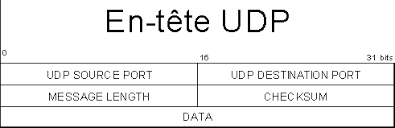
\includegraphics{image/udp.png}\\
remarque : Port source est facultatif : Si aucune réponse n'est attendue. \\
La somme de contrôle n'est pas seulement calculée sur l'en-tête et la donnée UDP un pseudo en-tête est pris en compte pour s'assurer que le datagramme arrive à la bonne destination. \\
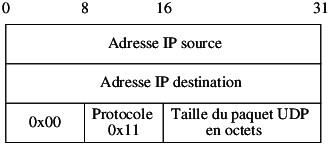
\includegraphics{image/udp2.png}
\newpage
\subsection{Fonctionnement général au niveau du system}
Si un datagramme UDP sur une machine sur un port p pas ouvert il envoie un massage ICMP port fermé. \\
Au niveau du système avec un port ouvertn le system va mettre en place un system de mémoire tampon et de file d'attente. Si aucun programme ne vient attraper les données, le tampon est saturé. \\
Si des nouveaux datagrammes arrivent certains seront détruits. \\
\\
Sula lecture des donnéesn il est possible que le système ne donne qu'une partie des données disponibles ou parvenues. \\
- read \\
- recu/ recufrom (?) \\
\\
L'UDP sera utile pour tout ce qui demande de la réactivité. \\
- Jeux vidéo \\
- Diffusion Audio/vidéo en direct \\

\section{\underline{TCP}}
 TCP pour Transfert Control Protocol, est un protocole orienté circuit c-à-d qu'il va essayer d'établir une connexion ( prendre contacte avec le destinataire, se mettre d'accord sur un certain sombres de paramètre). Si ça réussit un circuit virtuel est crée un flux de communication est mis en place. \\
Le flux est bidirectionnel et reste établie tant que les deux souhaitent conserver la connexion. \\
En terme de programmation ça ressemble à l'écriture ou la lecture sur un fichier. Ce flux de données est transcrits par IP. \\
Les données TCP vont être bufferisés (envoie/réception). Les données ne sont pas envoyer tout de suite au destinataire (pour limiter les échanges) les données reçus ne sont pas transmises directement au programme. \\
TCP effectue une remise fiable, c-à-d qu'il va garantit que tout message émis par une machine A va arriver à destination sur B. \\
Il doit exister une route entre A et B pendant la période de communication. \\
Le temps de communication va être raisonnable. \\
A l'émission d'un message de A vers B, TCP va attendre sur A de recevoir un accusé de réception de la part de B (Acknoledgement- ACK). \\ 
Scénario 1 : \\
\emph{Photo à insérer} \\
A envoie m à B. B le reçoit correctement et informe A de sa bonne réception.\\
Scénario 2 : \\
\emph{Photo à insérer} \\
A envoie m à B. Le message s'est perdu, A ré-envoie m à B et B informe la bonne réception de m.
Scénario 3 : \\
\emph{Photo à insérer} \\
A envoie m à B. B le reçois mais l'accusé de réception se perd, donc A ré-envoie le message et notifie de la bonne réception. \\
\newpage
Au niveau de TCP (de part et d'autre) à chaque fois qu'un message est envoyé, un timer sur la machine expéditeur est (?). Il correspond à la date limite de la réception de l'ACK. \\
\emph{Photo à insérer} \\
Si on envoie un message seulement quand l'ACK du message précédent nous parvient on va sous-utiliser le réseau. \\
\subsection{Fenêtre glissante (Sliding Windows)}
On a une valeur k (entier positif ou nul), k est envoyé avant de recevoir le premier accusé de réception. \\
\emph{Photo à insérer} \\
Que se passe-il quand A reçoit un ACK ? \\
On a le droit d'envoyer $m_{k+1}$.
\\ \emph{Photo à insérer} \\
Dans mon flux de données il y a 3 catégorie qui sont définis par rapport à la fenêtre.
Tout ce qui est à gauche de la fenêtre est bien reçu par B. \\
Tous ce qui est au milieu à été transmis à B et on ne sait pas encore s'il il est arrivé. \\
Tous ce qui est à droite est à transmettre mais pas encore expédier. \\
Les ACKs arrivent pas forcément dans l'ordre. \\
On peut envoyé $m_1,m_2,...m_k$ et recevoir $ACK_3$. \\
On ne débloque pas (encore) la fenêtre droite.
\subsection{Notion de port TCP}
TCP établie un circuit virtuel entre deux machines. Pour TCP, un serveur va attendre les connections sur un port donné. \\
Le circuit virtuel doit être établie entre les deux entités. Le serveur va accepter la connections du client et établir un circuit privé entre le client et le serveur.
\\ \emph{Photo à insérer} \\
Le serveur attend les connections et crée pour chaque demande de connections un circuit privé entre le client et le serveur. \\
\subsection{Contrôle de flux TCP}
TCP est orienté flux de données l'unité de base va être l'octet et TCP va acquitter chaque octet. \\ 
Le flux d'octet va être aussi géré par un mécanisme de fenêtre  glissante.
\\ \emph{Photo à insérer} \\
\\
On peut adapter le débit de la connections. \\
Le problème est que le débit du réseau utilise pas forcément le même que que les interfaces de A et de B. \\
PS : Le réseau peut être saturé. \\
Donc il est nécessaire d'adapter le débit. \\
\newpage
Comment peut-on augmenter le débit d'émission ? \\
On peut augmenter la fenêtre du coté droit. \\
\\
Comment peut-on limiter le débit d'émission ? \\
On baisse la fenêtre d'émission.\\
Mais on ne peut pas baisser la fenêtre droite car la limite droite est garantie. \\
Par contre à chaque fois qu'un message au début est acquitté. On ne déplace pas la limite droite d'une case quand la fenêtre contient k' messages (k' : Nouvelle longueur de fenêtre). \\
Remarque : La taille de la fenêtre peut passer à 0 -> Bloque la communication. \\
La réception peut envoyer une notification taille de fenêtre nul. \\

\subsection{Segment TCP}
[Équivalent aux datagrammes pour IP] \\
- Etablie la connections \\ 
- Fermer la connexion \\
- Envoie ACK \\
- Envoie message \\
- ... \\
\includegraphics{image/tcp.png} \\
\newpage
Certains segments partent des données et des infos pour le protocole. \\
Certains segments transportent seulement des informations de protocole. \\
\subsubsection{Établir la connections}
3 étapes : \\
- On veut obtenir une connections avec B.\\
\\ \emph{Photo à insérer} \\
Le premier message de $A$ pour $B$ avec une séquence $x$. $B$ répond avec SYN séquence $y$, ACK $x+1$. A envoie ACK $y+1$ la communication peut avoir lien. \\
\\
TCP refusera une demande ultérieur de connections entre un même hôte et un même destinataire (sur le même ports) si la connexion est toujours active. \\
\\
- Synchronisation \\
Une fois la connections établie; il faut initialiser les numéros de séquence pour la communication. Les deux étapes (connexion et synchronisation) se font en même temps avec l'envoie de SYN seq=$x$ et SYN seq=$y$. \\
\\
- Libération de connections \\
Cette dernière intervient quand les programmes ont terminés de communiquer (close()). \\
\emph{Photo à insérer} \\

Il est possible que pendant le processus de communication une ou plusieurs anomalie peuvent se produire et ne peuvent pas être récupérable. Une réinitialisation est donc nécessaire et a pour conséquence d'arrêter la transmission avec une fermeture brutale (Bit de code RST à 1). \\
\\
Le protocole TCP fonctionne avec un automate d'état fini.
\subsubsection{Données hors bande}
TCP fonctionne avec un flux de données. \\
Les communications sont "linéaires" pour envoyer l'octet x ; tous les octets précédents sont envoyés. \\
Si il est nécessaire d'envoyer des données urgentes, pour le protocole avec la notion de flux présenté, c'est pas possible. 
\\ 
Un mécanisme d'exception est prévu avec la notion de données urgente (Bit URG mis à 1). \\
Une procédure d'urgence indique où sont les données urgentes dans le flux. \\
Une fois les données traités, le programme/système revient en mode normal. \\
Les données urgentes sont nécessaires pour les tailles de fenêtre.
\newpage
\subsubsection{Taille des segments TCP}
La taille des segments est négociée à la connections MSS(Maximum Segment Size). pour que les systèmes puissent choisir des tailles de segments compatible avec leurs architectures et leurs contraintes. \\
Idéalement, en termes de taille de segment l'intérêt est que les segments ne soient pas fragmentés. Il y a quelques années le MSS optimal était évalué à 536 de manière \textbf{empirique\footnote{Statistiquement}}.
\subsubsection{Accusés de réceptions}
Précédemment on a vu que chaque message envoyé faisait l'objet d'accusé de réception. Si cette dernière n'était pas reçu avant l'expiration d'un timer, il fallait ré-expédier le message. \\
L'avantage d'être en version flux de données est que même si les ACKs se predent le protocole peut parfois continuer à fonctionner. \\
L'inconvénient c'est qu'on peut avoir à retransmettre l'intégralité des données.
\section{\underline{Protocole ICMP}}
ICMP pour Internet Control Message Protocol est un protocole d'erreur de IP (existe aussi pour IPv6). Il est indispensable au bon fonctionnement d'IP. ICMP se situe entre la couche 3 et la couche 4.
\subsection{Mode de fonctionnement}
Un message ICMP sera envoyé à chaque fois qu'un datagramme IP a un problème. ICMP transite sur le réseau par des datagrammes IP donc les messages d'erreur peuvent rencontrer des problèmes. Dans ce cas les messages ICMP ne provoquent de message d'erreurs. \\
ICMP envoie des messages, chaque message aura deux parties : \\
- En-tête (commune à tous les messages) \\
- Données (possiblement vides) \\

\subsection{Types de messages}
Sur 8 bits \\
0 : Réponse à une demande d'écho \\
3 : Destination inaccessible \\
4 : Limitation de la production de leur source \\
5 : Redirection \\
8 : Demande d'écho \\
9 : Annonce de routeur \\
10 : Sollicitation de routeur \\
11 : Expiration du délai \\
12 : Problème paramètres des données \\
13 : Demande d'horodatage \\ 
14 : Réponse à une demande d'horodatage \\
15 : Demande d'information réseau \\
16 : Réponse d'information réseau \\
17 : Demande masque sous réseau \\
18 : Réponse masque sous réseau \\
\\
Les types de message de 0 et 8 permettent de déterminer si l'hôte distant est accessible et si il est actifs. Ils permettent également de déterminer si l'hôte distant a les couches 1,2 et 3 fonctionnelles. 
\\ 
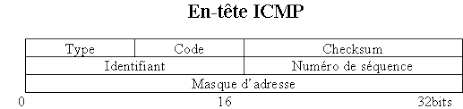
\includegraphics{image/icmp.png} 
\\
Pour les types de 0 à 8 le code est de 0. \\
Les données sont optionnels, il faut que ce soit identique à ce qui est reçu dans la réponse permet de savoir si des alterations des données sont intervenues. L'ID et le numéro de séquence permettent d'identifier chacune des demandes d'écho. 
\\

- Type 3 : Destination inaccessible. \\
Message envoyé lorsqu'un routeur n'est pas en mesure de faire parvenir un datagramme à destination. \\
Pour informer l'émetteur, le routeur rajoute les 64 premiers bits du datagramme concernés + l'entête IP. \\
\\

Code : \\
0 : Réseau inaccessible (problème de routage) \\
1 : Ordinateur inaccessible \\
2 : Protocole inaccessible \\
3 : Port inaccessible \\
4 : Fragmentation nécessaire mais DF (do not fragment) mis à 1. \\
5 : Échec de routage source \\ 
6 : Réseau de destination inconnue \\
7 : Ordinateur destination inconnue \\
8 : Ordinateur source isolé \\
9 : Communication avec le reseau destination interdit par l'administrateur \\
10 : Communication avec l'ordinateur destination interdit par l'administrateur \\ 
11 : Réseau inaccessible  (interdit) \\
12 : Ordinateur inaccessible (interdit) 
\\

- Type 4 Limitation de la production de la source. \\
Le routeur peut temporairement dans l'incapacité de traités toutes les requête. Pour ralentir l'émission des sources il peut envoyer un message de type 4 pour demander la réduction du débit d'émission chaque fois qu'un datagramme est détruit il envoie un message type 4 à la source. La source va réduire le débit (incitation mais pas obligation).
\\
\newpage

- Type 5 Redirection \\
Quand un routeur reçoit d'un ordinateur un datagramme à destination d'un réseau et que le routeur connait une meilleur route qui passe par lui. \\
Il indique à l'emetteur de s'adresser à un autre routeur. 
\\

Code : \\
0 : Redirection de donnée pour le réseau (le plus utilisé) \\
1 : Redirection pour un ordinateur \\
2 : Pour type de service et réseau \\
3 : Pour type de service et ordinateur \\
\\


- Type 11 Expiration de délai.
Pour limiter la durée de vie des datagrammes sur le réseau pour éviter l'engorgement inutile sir les tables de routages sont corrompus.
\\
Code : \\ 
0 : TTL expiré \\
1 : Réassemblage des datagrammes fragmentés 
\\
- Type 12 Problème paramètres des sonnées \\
Le datagramme doit être détruit à cause de ses options\\
\\

Code : \\
0 : \\
1 : Option obligatoire qui est absente un pointeur pointe sur l'option incorrecte. \\

\\

Type 13 et 14 Horodatage \\
Synchronisation horloge et estimation du temps . \\
Permet de demander l'heure à une machine/un routeur. \\
Type 13 : demande \\
Type 14 : réponse \\
\\
La demande part avec seulement l'horodatage d'émission. \\
Le récepteur en premier lieu il renseigne l'heure de réception \\
L'heure de transmission est indique au moment de l'émission \\
$\hookrightarrow$ Les temps sont indiqués en secondes depuis 1970. 
\subsection{Différents fonctionnement}
\end{document}
